\section[Puntos perpetuos enteros y extensiones Caputo]
{Puntos perpetuos: teoría entera, extensión Caputo y uso complementario}
\label{sec:perpetual-points}

\HAFOCardPerpetual

\subsection{Antecedentes, alcance y contraejemplos}

Prasad introdujo los puntos perpetuos para campos autónomos ordinarios como
puntos de velocidad no nula y aceleración nula
\cite{Prasad2015Perpetual}. Dudkowski, Prasad y Kapitaniak desarrollaron su uso
como condiciones iniciales para rastrear atractores coexistentes, incluidos
atractores raros u ocultos
\cite{DudkowskiPrasadKapitaniak2015,DudkowskiPrasadKapitaniak2017}, y estudios
posteriores compararon puntos regulares y perpetuos en varios tipos de
sistemas \cite{DudkowskiPrasadKapitaniak2018}.

La literatura también fija un límite decisivo. Nazarimehr, Saedi y Jafari
exhibieron sistemas en los cuales los puntos perpetuos no localizan el
atractor oculto \cite{NazarimehrSaediJafari2017}; Jafari, Nazarimehr y Sprott
mostraron que su sola existencia tampoco certifica disipatividad
\cite{JafariNazarimehrSprott2015}; y Nag Chowdhury y Ghosh presentaron un
sistema sin equilibrios cuyo atractor no se encuentra por esta vía
\cite{NagChowdhuryGhosh2020}. Por tanto, un PP es una semilla geométrica, no
una condición necesaria ni suficiente para un atractor oculto.

Las revisiones de atractores ocultos sitúan los PP entre los métodos de
localización \cite{DudkowskiEtAl2016,GuanXie2025}. Para Caputo se necesitan
dos construcciones distintas: una condición algebraica de arranque y un evento
dependiente de la historia. Su derivación debe conservar la memoria y evitar
una regla de cadena local inexistente.

\begin{table}[H]
\centering
\caption{Significado matemático de las construcciones.}
\label{tab:pp-status-map}
\small
\begin{tabularx}{\linewidth}{@{}L{0.30\linewidth}Y@{}}
\toprule
Construcción & Significado y alcance \\
\midrule
PP entero, \(Df(p)f(p)=0\), \(f(p)\ne0\) & Definición publicada y semilla
heurística con contraejemplos conocidos. \\
Caputo, Volterra, Picard, inicialización y L1 & Herramientas publicadas sobre
las que se construye la extensión. \\
FPP--A & Cancela el término local de orden
\(h^{2q}\); no es aceleración fraccionaria global. \\
FPP--H & Evento dependiente de la historia, no punto
intrínseco de \(\mathbb R^n\). \\
Caso inconmensurable y derivada de Bouligand/PWA & Condiciones que requieren
separar órdenes y regiones de suavidad. \\
\bottomrule
\end{tabularx}
\end{table}

\subsection{Derivación completa para una ODE autónoma}

Sea
\begin{equation}
 \dot x=f(x),\qquad x\in\Omega\subset\mathbb R^n,\qquad f\in C^1(\Omega).
 \label{eq:pp-ode}
\end{equation}
A lo largo de una solución clásica, la regla de la cadena da
\begin{equation}
 \ddot x(t)=\frac{d}{dt}f(x(t))
 =J_f(x(t))\dot x(t)=J_f(x(t))f(x(t)).
 \label{eq:pp-acceleration}
\end{equation}

\begin{definition}[punto perpetuo clásico]
Un punto \(p\in\Omega\) es perpetuo para \cref{eq:pp-ode} si
\begin{equation}
 J_f(p)f(p)=0,
 \qquad f(p)\neq0.
 \label{eq:pp-definition}
\end{equation}
La segunda condición excluye todos los equilibrios.
\end{definition}

El algoritmo algebraico consiste en resolver primero las \(n\) ecuaciones
\begin{equation}
 a(x):=J_f(x)f(x)=0,
 \label{eq:pp-algebraic-system}
\end{equation}
y después eliminar las raíces de \(f(x)=0\). No es suficiente resolver
\(\det J_f=0\), aunque esa ecuación es una criba necesaria.

\begin{proposition}[variedad singular necesaria]
Si \(p\) satisface \cref{eq:pp-definition}, entonces
\begin{equation}
 \det J_f(p)=0,
 \qquad f(p)\in\ker J_f(p)\setminus\{0\}.
 \label{eq:pp-singular-screen}
\end{equation}
\end{proposition}

\begin{proof}
Si \(J_f(p)\) fuera invertible, \(J_f(p)f(p)=0\) implicaría \(f(p)=0\), en
contradicción con la definición. Por ello \(J_f(p)\) es singular y el vector
no nulo \(f(p)\) pertenece a su núcleo.
\end{proof}

Así, una búsqueda eficiente puede intersectar la variedad
\(\det J_f=0\) con \(J_f f=0\), pero debe verificar las ecuaciones vectoriales
completas. En sistemas polinomiales se puede usar una base de Gröbner,
una descomposición triangular o eliminación real. Una resolución numérica
requiere precisión suficiente, aislamiento real y sustitución posterior;
un residuo pequeño por sí solo no demuestra exhaustividad.

La energía cinética de la velocidad de fase,
\begin{equation}
 K_f(x)=\frac12\|f(x)\|_2^2,
\end{equation}
satisface
\begin{equation}
 \frac{d}{dt}K_f(x(t))=f(x)^{\mathsf T}J_f(x)f(x).
 \label{eq:pp-speed-derivative}
\end{equation}
Todo PP hace estacionaria la rapidez, pero el recíproco es falso: la ecuación
escalar \(f^{\mathsf T}J_f f=0\) sólo exige ortogonalidad entre velocidad y
aceleración, no aceleración vectorial nula.

\subsection{Covariancia, coordenadas y campos no suaves}

Para un cambio afín invertible \(x=Ty+c\), el campo transformado es
\begin{equation}
 g(y)=T^{-1}f(Ty+c),\qquad J_g(y)=T^{-1}J_f(Ty+c)T,
\end{equation}
y, por tanto,
\begin{equation}
 J_g(y)g(y)=T^{-1}J_f(x)f(x).
 \label{eq:pp-affine-covariance}
\end{equation}
Los PP se transportan uno a uno bajo transformaciones afines. Bajo un
difeomorfismo no lineal \(x=h(y)\), en cambio,
\begin{equation}
 \ddot x=Dh(y)\ddot y+D^2h(y)[\dot y,\dot y],
 \label{eq:pp-nonlinear-coordinate}
\end{equation}
y el término Hessiano destruye la invariancia. Por eso los PP de PLL se
calculan en las coordenadas físicas publicadas, y una reformulación no lineal
de fase--velocidad debe considerarse otro experimento. Una versión
intrínsecamente geométrica requiere una conexión y aceleración covariante;
esa construcción y el transporte del desarrollo fraccionario se explican en
\cref{subsec:gt-connecting,subsec:gt-caputo-transfer}.

Los PP tampoco son invariantes bajo una reparametrización temporal dependiente
del estado. Si \(\widetilde f(x)=\alpha(x)f(x)\), \(\alpha(x)>0\), entonces
\begin{equation}
 J_{\widetilde f}\widetilde f
 =\alpha^2J_f f+\alpha f(\nabla\alpha\cdot f).
 \label{eq:pp-time-rescaling}
\end{equation}
Aunque las órbitas geométricas sean las mismas, el segundo término puede crear
o destruir PP. El conjunto pertenece a un campo y una escala temporal
concretos, no sólo a su retrato topológico.

Una generalización entera relacionada son las curvas de conexión
\begin{equation}
 J_f(x)f(x)=\lambda(x)f(x),
 \label{eq:pp-connecting-curves}
\end{equation}
que seleccionan velocidad y aceleración paralelas
\cite{GilmoreEtAl2010Connecting}. Los PP son el subconjunto
\(\lambda=0\), \(f\neq0\). Como la curva tiene normalmente dimensión mayor,
puede suministrar semillas donde no hay PP; trabajos posteriores la han usado
para localizar atractores ocultos \cite{GuanXie2021Connecting}. Su papel como
familia de semillas se desarrolla en \cref{subsec:gt-connecting}; no implica
que toda cuenca deba cortar una curva conectante.

En un campo PWA \(f_j(x)=A_jx+d_j\), los PP interiores de la región
\(\Omega_j\) satisfacen
\begin{equation}
 A_j(A_jx+d_j)=0,
 \quad A_jx+d_j\neq0,
 \quad x\in\operatorname{int}\Omega_j.
 \label{eq:pp-pwa-region}
\end{equation}
Una raíz algebraica fuera de su región se descarta. Sobre una superficie de
conmutación se necesitan aceleraciones laterales, una selección de Clarke o
una convención de Filippov; una igualdad obtenida con una derivada inexistente
no se clasifica como PP.

Para un sistema forzado \(\dot x=f(t,x)\), la aceleración es
\begin{equation}
 \ddot x=\partial_t f(t,x)+J_xf(t,x)f(t,x).
\end{equation}
Omitir \(\partial_t f\) cambia la definición. El análisis se restringe a
campos autónomos o a una extensión autónoma declarada con la fase del
forzamiento como estado adicional.

\subsection{Limitaciones de la extensión directa a Caputo}

Considérese ahora el PVI conmensurable
\begin{equation}
 {}^{\mathrm C}D_{t_0}^{q}x(t)=f(x(t)),
 \qquad x(t_0)=x_0,\qquad 0<q<1.
 \label{eq:pp-caputo-ivp}
\end{equation}
La siguiente regla de cadena local no es válida en general:
\begin{equation}
 {}^{\mathrm C}D^q[f(x(t))]
 \stackrel{\text{en general}}{\neq}
 J_f(x(t)){}^{\mathrm C}D^q x(t),
 \label{eq:pp-false-chain-rule}
\end{equation}
porque Caputo no posee esa regla de cadena local. Tampoco se puede identificar
sin condiciones
\begin{equation}
 {}^{\mathrm C}D^q({}^{\mathrm C}D^q x)
 \stackrel{\text{en general}}{\neq}
 {}^{\mathrm C}D^{2q}x.
 \label{eq:pp-no-semigroup}
\end{equation}
La transformada de Laplace del miembro izquierdo incluye los datos iniciales
del primer operador y de \({}^{\mathrm C}D^qx\); el operador de orden \(2q\)
usa otro conjunto de términos iniciales, que además cambia cuando
\(2q\) cruza uno.

Dos cálculos elementales hacen visible la falla. Para \(x(t)=t^q\) y
\(\phi(u)=u^2\),
\begin{align}
 {}^{\mathrm C}D_0^q[x(t)^2]
 &=\frac{\Gamma(2q+1)}{\Gamma(q+1)}t^q,\\
 2x(t){}^{\mathrm C}D_0^qx(t)
 &=2\Gamma(q+1)t^q.
 \label{eq:pp-chain-counterexample}
\end{align}
Para \(q=1/2\) resultan, respectivamente,
\(2t^{1/2}/\sqrt\pi\) y \(\sqrt\pi t^{1/2}\). Las reglas de composición
fraccionarias contienen memoria o series adicionales
\cite{ShchedrinEtAl2018Composite}.

Para la composición, sea \(q=1/3\), \(x(t)=t^{1/3}\). Entonces
\begin{equation}
 {}^{\mathrm C}D_0^{1/3}x=\Gamma(4/3),\qquad
 {}^{\mathrm C}D_0^{1/3}({}^{\mathrm C}D_0^{1/3}x)=0,
\end{equation}
mientras
\begin{equation}
 {}^{\mathrm C}D_0^{2/3}x
 =\frac{\Gamma(4/3)}{\Gamma(2/3)}t^{-1/3}\neq0.
 \label{eq:pp-semigroup-counterexample}
\end{equation}
Las propiedades parciales de semigrupo requieren dominios e hipótesis
específicas \cite{Cong2023Semigroup}.

La solución genérica tampoco es \(C^2\) en el terminal inferior. Si
\(f(x_0)\neq0\), el primer término es proporcional a
\((t-t_0)^q\), cuya derivada ordinaria es singular para \(q<1\). Por ello,
\(\ddot x(t_0)\) no es un sustituto consistente.

Un contraejemplo mínimo es el campo constante \(f(x)=c\neq0\). La solución es
\begin{equation}
 x(t)=x_0+\frac{c(t-t_0)^q}{\Gamma(q+1)}.
 \label{eq:pp-constant-field-solution}
\end{equation}
La derivada secuencial del campo y la derivada ordinaria de la solución dan
\begin{equation}
 {}^{\mathrm C}D^q[c]=0,
 \qquad
 \frac{d^2x}{dt^2}
 =\frac{c(t-t_0)^{q-2}}{\Gamma(q-1)}\neq0.
 \label{eq:pp-constant-field-counterexample}
\end{equation}
Así, ``aceleración secuencial fraccionaria'', aceleración ordinaria y
\(J_f f\) son objetos diferentes.

Además, un PVI de Caputo no genera en general un flujo ordinario sobre
\(\mathbb R^n\): el futuro necesita información heredada y soluciones
distintas pueden compartir un estado puntual. Una semidinámica rigurosa se
construye en un espacio funcional de historias
\cite{CongTuan2017Nonlocal,DoanKloeden2021Semidynamical}. Por último, para un
terminal inferior finito y las hipótesis autónomas usuales, no existen
soluciones no constantes exactamente periódicas
\cite{TavazoeiHaeri2009,KaslikSivasundaram2012}. En las figuras fraccionarias
debe decirse oscilación acotada, recurrencia o periodicidad aparente en ventana
finita, salvo que se cambie el operador o su terminal inferior.

\subsection{FPP--A: semilla algebraica de arranque Picard--Caputo}

La ecuación integral equivalente a \cref{eq:pp-caputo-ivp} es
\begin{equation}
 x(t_0+h)=x_0+\frac1{\Gamma(q)}
 \int_0^h(h-\tau)^{q-1}f(x(t_0+\tau))\,d\tau.
 \label{eq:pp-caputo-volterra-local}
\end{equation}
Para \(f\in C^2\) en una vecindad de \(x_0\), tome un intervalo local
donde la solución permanezca en ella y \(\|f\|\le M\). La ecuación
integral da primero
\(\|x(t_0+h)-x_0\|\le Mh^q/\Gamma(q+1)\). Como \(f\) es localmente
Lipschitz, \(f(x(t_0+h))=f_0+O(h^q)\), y una segunda sustitución produce
\(x-x_0=f_0h^q/\Gamma(q+1)+O(h^{2q})\). Al insertar esta expresión en
el desarrollo de Taylor de \(f\), con \(f_0=f(x_0)\), \(J_0=J_f(x_0)\),
se obtiene
\begin{equation}
 x(t_0+h)=x_0+
 \frac{h^q}{\Gamma(q+1)}f_0+
 \frac{h^{2q}}{\Gamma(2q+1)}J_0 f_0+
 O(h^{3q}).
 \label{eq:pp-picard-expansion}
\end{equation}
El segundo coeficiente se obtiene de
\begin{align}
 f(x(t_0+\tau))
 &=f_0+J_0\frac{\tau^q}{\Gamma(q+1)}f_0+O(\tau^{2q}),\\
 I^q[\tau^q]
 &=\frac{\Gamma(q+1)}{\Gamma(2q+1)}h^{2q}.
\end{align}
En efecto, el cambio \(\tau=h\xi\) en la integral transforma el
coeficiente en \(B(q,q+1)/\Gamma(q)\). Análogamente, integrar un resto
acotado por \(C\tau^{2q}\) lo acota por
\(C\Gamma(2q+1)h^{3q}/\Gamma(3q+1)\). Así se justifica el orden del
resto sin diferenciarlo ni componer derivadas de Caputo.
Por tanto, \(J_0 f_0=0\) cancela la primera curvatura no trivial de la serie
Picard fraccionaria.

Con sólo \(f\in C^1\), la consecuencia robusta es
\begin{equation}
 \lim_{h\downarrow0}
 \Gamma(q+1)
 \frac{f(x(t_0+h))-f(x_0)}{h^q}
 =J_f(x_0)f(x_0).
 \label{eq:pp-startup-limit}
\end{equation}
En efecto,
\(x(t_0+h)-x_0=h^qf_0/\Gamma(q+1)+o(h^q)\), y la
diferenciabilidad de \(f\) completa el límite.

\begin{definition}[semilla perpetua Picard--Caputo, FPP--A]
Un estado \(p\) es una semilla FPP--A si
\begin{equation}
 J_f(p)f(p)=0,\qquad f(p)\neq0.
 \label{eq:fppa-definition}
\end{equation}
En \(q<1\), la condición significa que el término \(h^{2q}\) de
\cref{eq:pp-picard-expansion} se anula, o equivalentemente que el límite de
\cref{eq:pp-startup-limit} es cero. No significa aceleración fraccionaria
global nula.
\end{definition}

El conjunto FPP--A es independiente de \(q\): el orden cambia la salida
temporal desde la semilla, no las raíces de \(J_f f\). Esto es una ventaja
computacional y también una limitación; por sí solo no selecciona qué orden
fraccionario sostendrá un atractor.

Para desempatar raíces, \(f\in C^2\) permite desarrollar también la velocidad
fraccionaria:
\begin{align}
 f(x(t_0+h))
 ={}&f_0+\frac{J_0 f_0}{\Gamma(q+1)}h^q\\
 &+\left[
 \frac{J_0^2f_0}{\Gamma(2q+1)}
 +\frac{D^2f(x_0)[f_0,f_0]}{2\Gamma(q+1)^2}
 \right]h^{2q}+o(h^{2q}).
 \label{eq:pp-fractional-velocity-second}
\end{align}
En una FPP--A, \(J_0 f_0=0\), y queda
\begin{equation}
 f(x(t_0+h))-f_0
 =\frac{D^2f(x_0)[f_0,f_0]}{2\Gamma(q+1)^2}h^{2q}
 +o(h^{2q}).
 \label{eq:pp-hessian-tiebreaker}
\end{equation}
La norma del coeficiente Hessiano permite ordenar semillas. Si ese vector
es no nulo, \cref{eq:pp-hessian-tiebreaker} predice una pendiente log--log
\(2q\); si también se anula, hay que calcular un término de orden superior
y no se puede asignar esa pendiente. Ninguna de estas pruebas constituye
estabilidad de Lyapunov, pues una FPP no es un equilibrio.

\subsection{FPP--H: evento perpetuo dependiente de historia}

Definimos la velocidad fraccionaria a lo largo de una trayectoria por
\begin{equation}
 v_q(t):={}^{\mathrm C}D_{t_0}^qx(t)=f(x(t)).
\end{equation}
Si \(v_q\) es absolutamente continua en el intervalo considerado, su
aceleración secuencial es
\begin{align}
 \mathcal A_{q,q}[x](t)
 &:={}^{\mathrm C}D_{t_0}^qv_q(t)
 ={}^{\mathrm C}D_{t_0}^q[f(x(\cdot))](t)
 \label{eq:fpph-sequential-definition}\\
 &=\frac1{\Gamma(1-q)}
 \int_{t_0}^{t}(t-\tau)^{-q}
 \frac{d}{d\tau}f(x(\tau))\,d\tau.
 \label{eq:fpph-history-integral}
\end{align}

\begin{definition}[evento perpetuo Caputo, FPP--H]
Una pareja estado--historia \((x(t_\star),\mathcal H_{t_\star})\), con
\(t_\star>t_0\) y derivada secuencial finita y definida, es un evento
FPP--H si
\begin{equation}
 \mathcal A_{q,q}[x](t_\star)=0,
 \qquad f(x(t_\star))\neq0.
 \label{eq:fpph-event}
\end{equation}
\end{definition}

No es, en general, un punto del espacio de estados. Dos historias que llegan
al mismo \(x(t_\star)\) pueden producir valores diferentes de
\(\mathcal A_{q,q}\). Para \(q=1\), el operador se define como la
derivada ordinaria de \(f(x(t))\), igual a \(J_f(x)f(x)\), y recupera
la definición clásica. No se sustituye \(q=1\) directamente en la
integral con prefactor \(1/\Gamma(1-q)\), válida para \(0<q<1\).

Hay una clase exacta adicional. Si \(f(x)=Ax+d\) globalmente, la linealidad de
Caputo implica
\begin{equation}
 {}^{\mathrm C}D^q[f(x(t))]
 =A{}^{\mathrm C}D^qx(t)=A(Ax(t)+d).
 \label{eq:pp-affine-exact-caputo}
\end{equation}
Por ello FPP--A y FPP--H coinciden para campos afines globales. En PWA, esta
identidad sólo vale si toda la historia relevante permanece en la misma
región; cruzar una frontera conserva contribuciones de ambos campos.

\subsection{Órdenes inconmensurables y extensión direccional}

Para
\begin{equation}
 {}^{\mathrm C}D_{t_0}^{q_j}x_j=f_j(x),\qquad 0<q_j<1,
 \label{eq:pp-incommensurate}
\end{equation}
con \(f\in C^1\) cerca del dato inicial, sea \(q_\star=\min_jq_j\) y
sea \(P_\star\) la matriz diagonal que selecciona
las componentes con \(q_j=q_\star\). La ecuación integral componente a
componente da
\(x_j(t_0+h)-x_{0j}=f_j(x_0)h^{q_j}/\Gamma(q_j+1)+o(h^{q_j})\).
Al dividir el incremento vectorial entre \(h^{q_\star}\), las componentes
con \(q_j>q_\star\) tienden a cero. Aplicar Taylor de primer orden a
\(f\) produce
\begin{equation}
 f(x(t_0+h))-f(x_0)
 =\frac{h^{q_\star}}{\Gamma(q_\star+1)}
 J_f(x_0)P_\star f(x_0)+o(h^{q_\star}).
 \label{eq:pp-incommensurate-leading}
\end{equation}
La condición de cancelación del término dominante es
\begin{equation}
 J_f(x_0)P_\star f(x_0)=0,
 \label{eq:pp-incommensurate-condition}
\end{equation}
no \(J_f f=0\). Si se anula, el siguiente exponente depende de los demás
\(q_j\), de \(2q_\star\) y de resonancias entre órdenes. Por esa razón, el
protocolo ejecutable inicial se restringe a órdenes conmensurables; el caso
inconmensurable es una extensión teórica propuesta.

Si \(f\) es localmente Lipschitz y direccionalmente diferenciable en el
sentido de Bouligand, el incremento inicial es
\(h^q f(x_0)/\Gamma(q+1)+o(h^q)\). La propiedad Lipschitz hace que
el término \(o(h^q)\) cambie \(f\) sólo en \(o(h^q)\); la homogeneidad
positiva de la derivada direccional identifica el límite de arranque con
\(f'(x_0;f(x_0))\). La condición de cancelación es, por tanto,
\begin{equation}
 f'(x_0;f(x_0))=0,\qquad f(x_0)\neq0.
 \label{eq:pp-bouligand}
\end{equation}
En un campo continuo PWA se usa la región hacia la que apunta \(f(x_0)\).
Si el vector es tangente a una única frontera plana, los campos afines
coinciden sobre ella y sus derivadas en esa dirección también coinciden;
el producto lateral común define entonces la derivada. En otros puntos
tangentes o intersecciones se comprueba directamente que el límite exista,
como se hace para Muñoz--Pacheco. Campos discontinuos y deslizamiento de
Filippov requieren otra convención y quedan fuera de esta construcción.

\subsection{Aproximación L1 y criterio numérico de evento}

Sea \(g_n=f(x_n)\) sobre una malla uniforme \(t_n=t_0+nh\). La aproximación L1
de \cref{eq:fpph-sequential-definition} es
\begin{equation}
 \mathcal A_{q,n}^{L1}
 =\frac1{\Gamma(2-q)h^q}
 \sum_{j=0}^{n-1}
 \left[(j+1)^{1-q}-j^{1-q}\right]
 (g_{n-j}-g_{n-j-1}).
 \label{eq:fpph-l1}
\end{equation}
El diagnóstico normalizado usado en el experimento numérico es
\begin{equation}
 \eta_{q,n}
 =\frac{\|\mathcal A_{q,n}^{L1}\|_2}{1+\|f(x_n)\|_2}.
 \label{eq:fpph-normalized}
\end{equation}
Se excluye un intervalo de arranque, se buscan mínimos locales y se exige
\(\|f(x_n)\|>\nu\). Un cero vectorial a lo largo de una curva unidimensional
no es genérico; por eso su clasificación como evento requiere que el mínimo y
la trayectoria converjan al usar \(h,h/2\) y, en una ventana corta, \(h/4\), siempre con el
mismo terminal inferior y la misma política de memoria. Un umbral visual no
es suficiente.

Al localizar un mínimo se ejecutan dos experimentos distintos:
\begin{enumerate}
 \item continuar la trayectoria portadora con toda su historia;
 \item iniciar un PVI nuevo desde \(x(t_\star)\) con historia reiniciada.
\end{enumerate}
El segundo no comprueba el mismo evento FPP--H; evalúa si el estado aislado es
una semilla útil. Ambos resultados deben conservarse.

\subsection{Cuenca de reinicio y cuenca en el espacio de memoria}

Sea \(X_{\mathrm{adm}}\) un espacio invariante de historias admisibles,
con existencia global y continuidad de la semidinámica justificadas y con
la topología relativa declarada. Sea \(\phi_e\) la historia constante de un
equilibrio \(e\). Un concepto fuerte de ocultedad requeriría que para cada
equilibrio exista una vecindad abierta \(\mathcal U_e\) tal que
\begin{equation}
 \mathcal U_e\cap\mathcal B_{X_{\mathrm{adm}}}(\mathcal A)=\varnothing.
 \label{eq:pp-functional-hiddenness}
\end{equation}
En cómputo se explora normalmente sólo una inmersión de reinicio
\(\iota:\mathbb R^n\to X_{\mathrm{adm}}\), que asigna al estado puntual la
prehistoria prescrita. La cuenca observada es entonces
\begin{equation}
 \mathcal B_{\mathrm{reset}}(\mathcal A)
 =\iota^{-1}[\mathcal B_{X_{\mathrm{adm}}}(\mathcal A)].
 \label{eq:pp-reset-section-basin}
\end{equation}
Si no se admiten todos los estados, se restringe el dominio de \(\iota\).
La continuidad de esta aplicación hace que la exclusión de una vecindad
relativa funcional implique la exclusión de su corte de reinicio; la
recíproca no se deduce. No se toma automáticamente
\(X_{\mathrm{adm}}=C([0,\infty),\mathbb R^n)\): la
\cref{prop:geofo-full-space-obstruction} demuestra la obstrucción a la
atracción abierta y a la exclusión de vecindades en ese espacio completo.
Los sondeos finitos aportan evidencia sobre las condiciones de reinicio
muestreadas, sin certificar toda la cuenca de reinicio ni
\cref{eq:pp-functional-hiddenness}.

\subsection{Ejemplo entero publicado para verificación}

Un ejemplo algebraicamente cerrado de la literatura es
\begin{align}
 \dot x&=y,\\
 \dot y&=z,\\
 \dot z&=-y+3y^2-x^2-xz+\alpha.
 \label{eq:pp-prasad-system}
\end{align}
Si \(F=-y+3y^2-x^2-xz+\alpha\), entonces
\begin{equation}
 f=\begin{pmatrix}y\\z\\F\end{pmatrix},\qquad
 J_f=\begin{pmatrix}
 0&1&0\\0&0&1\\-2x-z&-1+6y&-x
 \end{pmatrix},
\end{equation}
y la multiplicación completa es
\begin{equation}
 J_f f=\begin{pmatrix}
 z\\F\\(-2x-z)y+(-1+6y)z-xF
 \end{pmatrix}.
 \label{eq:pp-prasad-acceleration}
\end{equation}
Para \(\alpha<0\), \(J_f f=0\) implica sucesivamente
\(z=0\), \(F=0\) y \(-2xy=0\). La rama \(y=0\) exigiría
\(x^2=\alpha<0\); por ello \(x=0\) y
\begin{equation}
 p_\pm=
 \left(0,\frac{1\pm\sqrt{1-12\alpha}}6,0\right).
 \label{eq:pp-prasad-roots}
\end{equation}
Con \(\alpha=-0.05\), las coordenadas \(y\) son
\(-0.044151844013\ldots\) y \(0.377485177347\ldots\). En ambas,
\(f=(y,0,0)^\mathsf T\neq0\). La literatura reporta destinos diferentes:
la raíz positiva localiza el atractor oculto y la negativa produce una órbita
no acotada \cite{Prasad2015Perpetual,DudkowskiPrasadKapitaniak2018}. Es una
comparación entre una semilla que localiza el atractor y otra que diverge.

En estas raíces,
\begin{equation}
 D^2f(p_\pm)[f(p_\pm),f(p_\pm)]
 =(0,0,-2y_\pm^2)^\mathsf T,
\end{equation}
por lo que \cref{eq:pp-hessian-tiebreaker} predice
\begin{equation}
 f(x(t_0+h))-f(p_\pm)
 =\left(0,0,-\frac{y_\pm^2}{\Gamma(q+1)^2}h^{2q}\right)^\mathsf T
 +o(h^{2q}).
 \label{eq:pp-prasad-caputo-prediction}
\end{equation}
La pendiente \(2q\) es una prueba numérica directa de la traducción Caputo.

\subsection{Resolución algebraica en los sistemas analizados}
\label{sec:pp-case-audit}

Se resolvió \(J_f f=0\) con álgebra simbólica, se eliminaron los
equilibrios, se sustituyó cada raíz a precisión alta y se comprobaron las
regiones PWA y las simetrías. La
\cref{tab:pp-case-map} resume el resultado; después se muestran las
derivaciones representativas.

\begin{longtable}{@{}L{0.20\linewidth}L{0.25\linewidth}L{0.25\linewidth}L{0.22\linewidth}@{}}
\caption{Aplicabilidad de puntos perpetuos en los sistemas analizados.}
\label{tab:pp-case-map}\\
\toprule
Caso & Raíces no estacionarias & Función & Resultado dinámico\\
\midrule
\endfirsthead
\toprule
Caso & Raíces no estacionarias & Función & Resultado dinámico\\
\midrule
\endhead
Chua PWL & Ninguna regional; tampoco en \(x=\pm1\) lateralmente & Control
negativo; localizar por DF u otra familia de semillas & Ausencia de PP
demostrada.\\
Chua arctan Wu & Un par simétrico & Semillas FPP--A fraccionarias &
Trayectorias acotadas; destino asintótico sin resolver.\\
Chua arctan c590 & Un par muy lejano, con \(\|f\|\approx545\) & Control de
divergencia y de semillas inadecuadas & Dinámica de estas semillas sin resolver.\\
Kalman--Fitts & Ninguna, porque \(\det J_f=0.98191881\) & Control negativo de
la condición singular necesaria & Sin PP; ciclo localizado por conmutación.\\
Jerk cuadrático & Ninguna & Control de realizaciones M1 & Ausencia de PP
demostrada.\\
Jerk exponencial & Ninguna & Control de realizaciones escalares & Ausencia
de PP y FPP--A conmensurables demostrada.\\
MAVPD & Dos raíces cerradas por parámetro & Localización de ciclos interiores &
Trayectorias recurrentes; control de horizonte incompleto.\\
PLL lead--lag & Dos raíces por vuelta del cilindro & Comparar con órbita
corredora en coordenadas físicas & Una semilla llega al foco; la otra
permanece transitoria.\\
Lorenz generalizado \(q=0.995\) & Dos raíces no estacionarias & Segundo experimento
fraccionario multicanal & Raíces algebraicas; destino dinámico sin resolver.\\
Rabinovich--Fabrikant \(q=0.998\) & Ocho raíces en cuatro pares & Caso de referencia MIMO
con reducción por simetría & Raíces algebraicas; destino dinámico sin resolver.\\
Muñoz--Pacheco \(q=0.97\) & Cuatro raíces suaves; recta direccional & Experimento preliminar Caputo
FPP--A/FPP--H & Trayectorias finitas con ABM de memoria completa.\\
\bottomrule
\end{longtable}

\subsubsection{MAVPD: solución cerrada y experimento preliminar entero}

Para
\begin{equation}
 f(u,v,w)=
 \begin{pmatrix}
 \delta(\gamma u+v-u^3)\\u-\xi v-w\\\rho v
 \end{pmatrix},
 \label{eq:pp-mavpd-field}
\end{equation}
la tercera fila de \(J_f f=0\) da \(\rho f_2=0\), luego \(f_2=0\). La segunda
fila reduce a \(f_1-f_3=0\), esto es \(f_1=\rho v\). La primera fila es
\begin{equation}
 \delta(\gamma-3u^2)f_1+\delta f_2=0.
\end{equation}
Para una raíz no estacionaria \(f_1\neq0\), se obtiene
\(u^2=\gamma/3\). Sustituyendo en \(f_1=\rho v\),
\begin{equation}
 u_\star=\pm\sqrt{\frac\gamma3},\qquad
 v_\star=\frac{2\delta\gamma u_\star}{3(\rho-\delta)},
 \qquad w_\star=u_\star-\xi v_\star,
 \label{eq:pp-mavpd-closed}
\end{equation}
con \(\delta\rho\ne0\), \(\gamma>0\) y \(\rho\neq\delta\). Para
\(\delta=100,\rho=200,\gamma=0.1,\xi=3.1\),
\begin{equation}
 p_\pm=\pm(0.1825741858350554,
 0.01217161238900369,0.1448421874291439).
\end{equation}
La sustitución da \(J_f(p_\pm)f(p_\pm)=0\) exactamente y
\(\|f(p_\pm)\|=3.44265186329548\).

El experimento DOP853, \(t\in[0,120]\), con tolerancias
\(10^{-10}/10^{-12}\), llegó desde ambos PP a las órbitas periódicas
simétricas ya conocidas del análisis. En \(t\ge80\) los rangos fueron
\((0.37943,0.05722,0.97545)\). El detector registró 74 y 75 máximos, periodos
medios \(0.53760\) y \(0.53730\), y coeficientes de variación \(0.0361\) y
\(0.0223\), respectivamente. Así, la clasificación periódica queda
respaldada por estos diagnósticos a tiempo finito. La persistencia al aumentar
el horizonte y la relación con otras cuencas se examinan en
\cref{sec:resultados-piloto-gt}.

\begin{hafocommonfigure}[H]
 \centering
 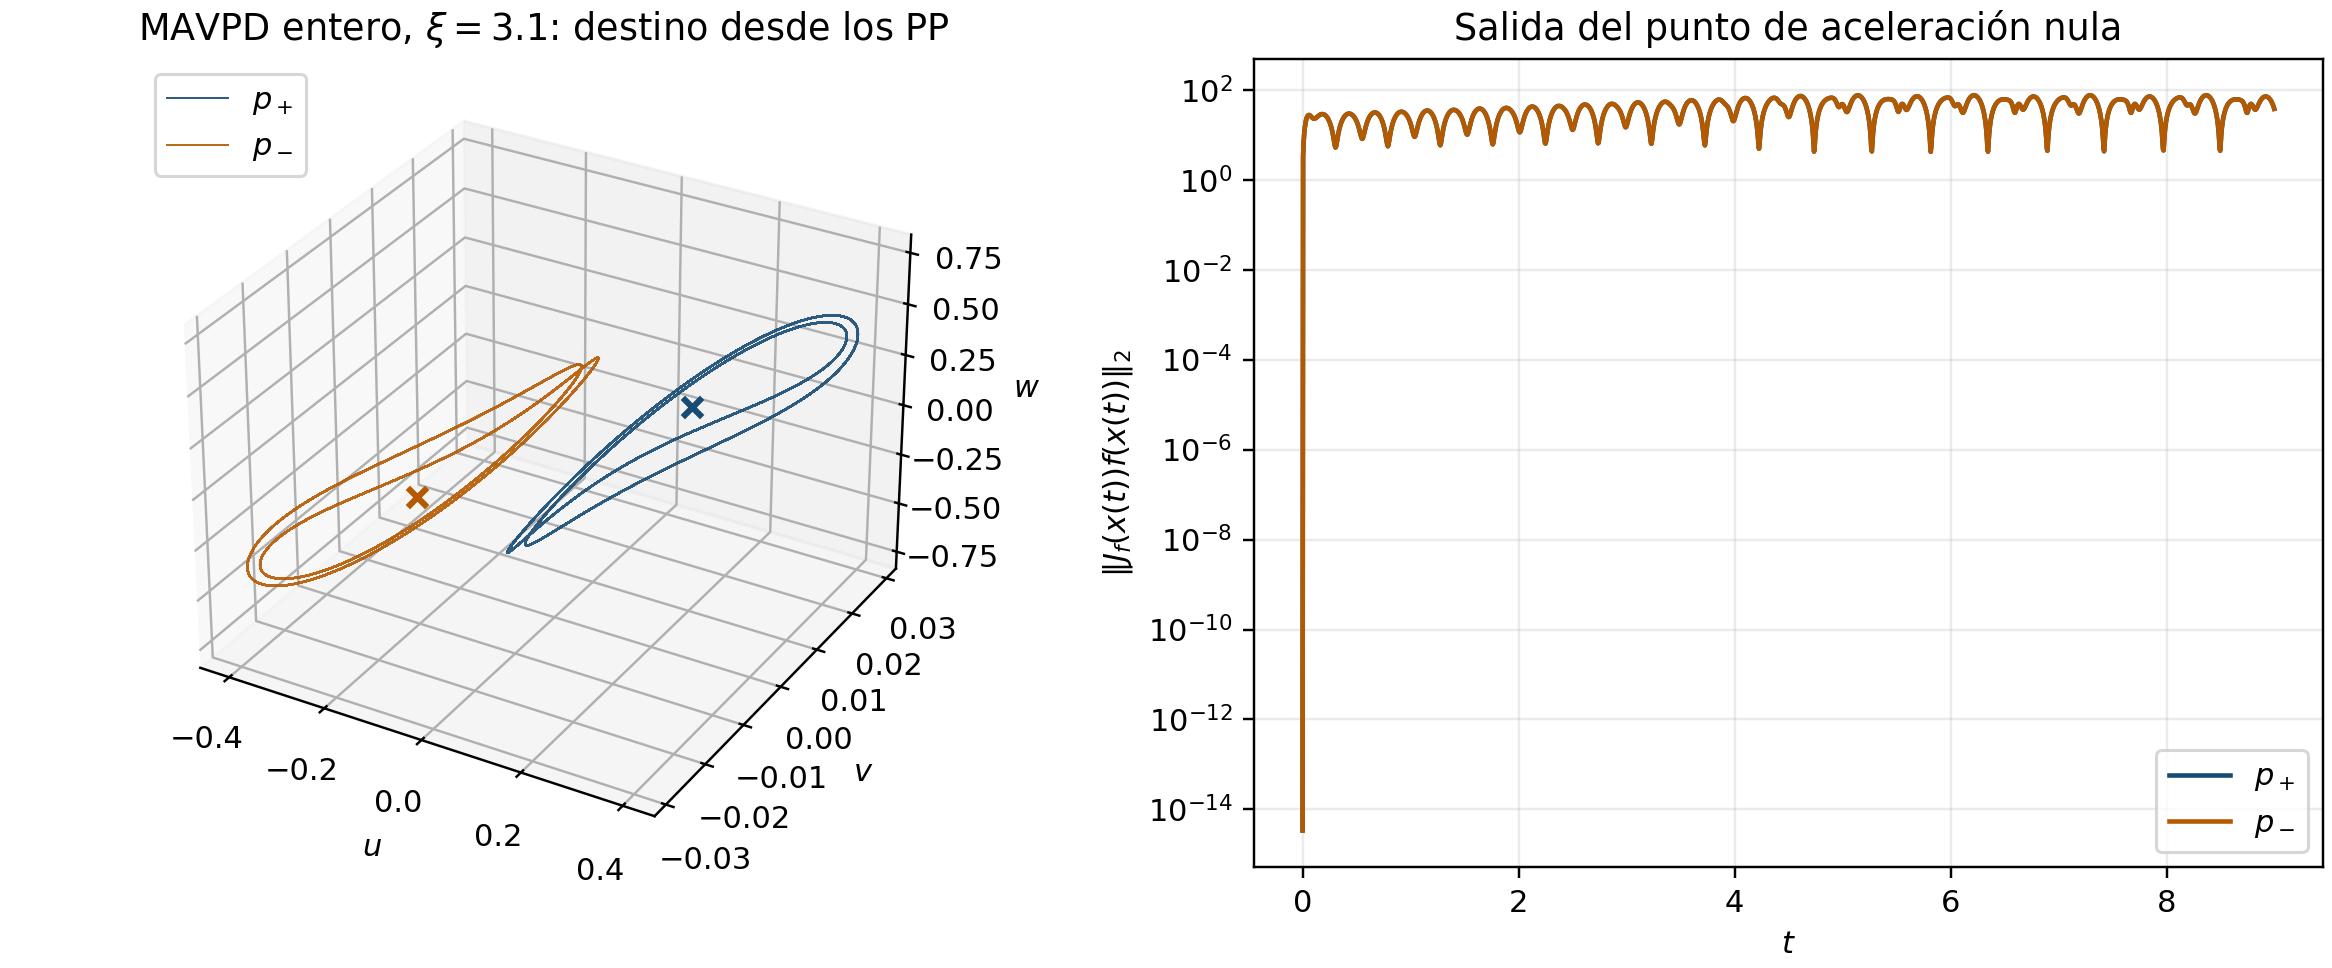
\includegraphics[width=0.98\linewidth]{figures/perpetual/perpetual_mavpd_integer.png}
 \caption{Experimento PP entero en MAVPD, \(\xi=3.1\). Las cruces son los PP
 exactos; las curvas son los destinos después del transitorio. El panel
 derecho muestra que \(J_f f=0\) sólo en el instante inicial y no a lo largo de
 toda la órbita.}
 \label{fig:pp-mavpd-pilot}
\end{hafocommonfigure}

\subsubsection{Muñoz--Pacheco: raíces suaves y frontera no diferenciable}

Para
\begin{equation}
 f(x,y,z)=
 \begin{pmatrix}
 yz+x(y-a)\\1-|x|\\-xy-z
 \end{pmatrix},\qquad a=0.35,
 \label{eq:pp-munoz-field}
\end{equation}
se trabaja por regiones \(s=\operatorname{sign}x\):
\begin{equation}
 J_f=
 \begin{pmatrix}
 y-a&z+x&y\\-s&0&0\\-y&-x&-1
 \end{pmatrix}.
 \label{eq:pp-munoz-jacobian}
\end{equation}
La segunda ecuación de \(J_f f=0\) impone \(f_1=0\). La tercera da
\(f_3=-xf_2\), y la primera se convierte en
\begin{equation}
 f_2(z+x-xy)=0.
\end{equation}
Como \(f_2=0\) llevaría a un equilibrio, se excluye esa rama. En efecto,
\(f_2=0\) exige \(|x|=1\), \(f_3=0\) da \(z=-xy\), y entonces
\[
 f_1=-x(y^2-y+a)
 =-x\bigl[(y-\tfrac12)^2+a-\tfrac14\bigr]\ne0
\]
para $a=0.35>1/4$ y $x=\pm1$; no hay equilibrios. Se obtiene
\(z=x(y-1)\). Usando
\(f_3=-xy-z=-xf_2\), resulta
\begin{equation}
 y=1-\frac{|x|}{2}.
\end{equation}
Finalmente, \(f_1=0\) reduce a \(x(y^2-a)=0\), de modo que
\begin{equation}
 y=\varepsilon\sqrt a,\qquad
 u_\varepsilon=2(1-\varepsilon\sqrt a),\qquad
 (x,y,z)=
 \left(su_\varepsilon,\varepsilon\sqrt a,
 -\frac{s u_\varepsilon^2}{2}\right),
 \label{eq:pp-munoz-closed}
\end{equation}
para \(\varepsilon,s\in\{\pm1\}\). Numéricamente:
\begin{align}
 &(\pm0.816784043380077, 0.591607978309962,
 \mp0.333568086760154),\\
 &(\pm3.183215956619923, -0.591607978309962,
 \mp5.066431913239846).
\end{align}
El residuo vectorial se anula exactamente; las normas del campo son
\(0.2365640964\) y \(7.2845066702\). Todas las raíces están separadas de
\(x=0\), por lo que la derivada regional de \(|x|\) es válida.

En la frontera \(x=0\) no existe un Jacobiano clásico único. El criterio
direccional de \cref{eq:pp-bouligand} debe evaluarse por separado.
Allí \(f=(yz,1,-z)^{\mathsf T}\), y la segunda componente de la
derivada en la dirección \(f\) es \(-|yz|\). Su anulación exige
\(yz=0\); si \(z\ne0\), se tendría \(y=0\) y la tercera componente
sería \(z\ne0\). Por tanto, las únicas raíces direccionales de frontera
son \((0,y,0)\). Ambos Jacobianos laterales también anulan \(f\) sobre
esa recta. Sin embargo, sus soluciones exactas son
\begin{equation}
 x(t)=z(t)=0,\qquad
 y(t)=y_0+\frac{(t-t_0)^q}{\Gamma(q+1)},\qquad 0<q\le1.
 \label{eq:pp-munoz-boundary-orbit}
\end{equation}
La sustitución en la ecuación de Volterra comprueba la solución. Son
trayectorias no acotadas; las cuatro raíces anteriores agotan los PP de las
regiones suaves, pero no las raíces del criterio direccional de frontera.

El experimento Caputo usó \(q=0.97\), PECE de Diethelm con historia completa,
\(h=0.01\) y \(t_f=35\). Las cuatro trayectorias permanecieron finitas; las
normas máximas fueron \(6.421\) para el par interior y \(10.178\) para el
exterior. Los rangos no triviales no certifican un atractor ni caos: son
diagnósticos finitos que deben contrastarse al refinar paso y horizonte.

\begin{hafodigitalfigure}[H]
 \centering
 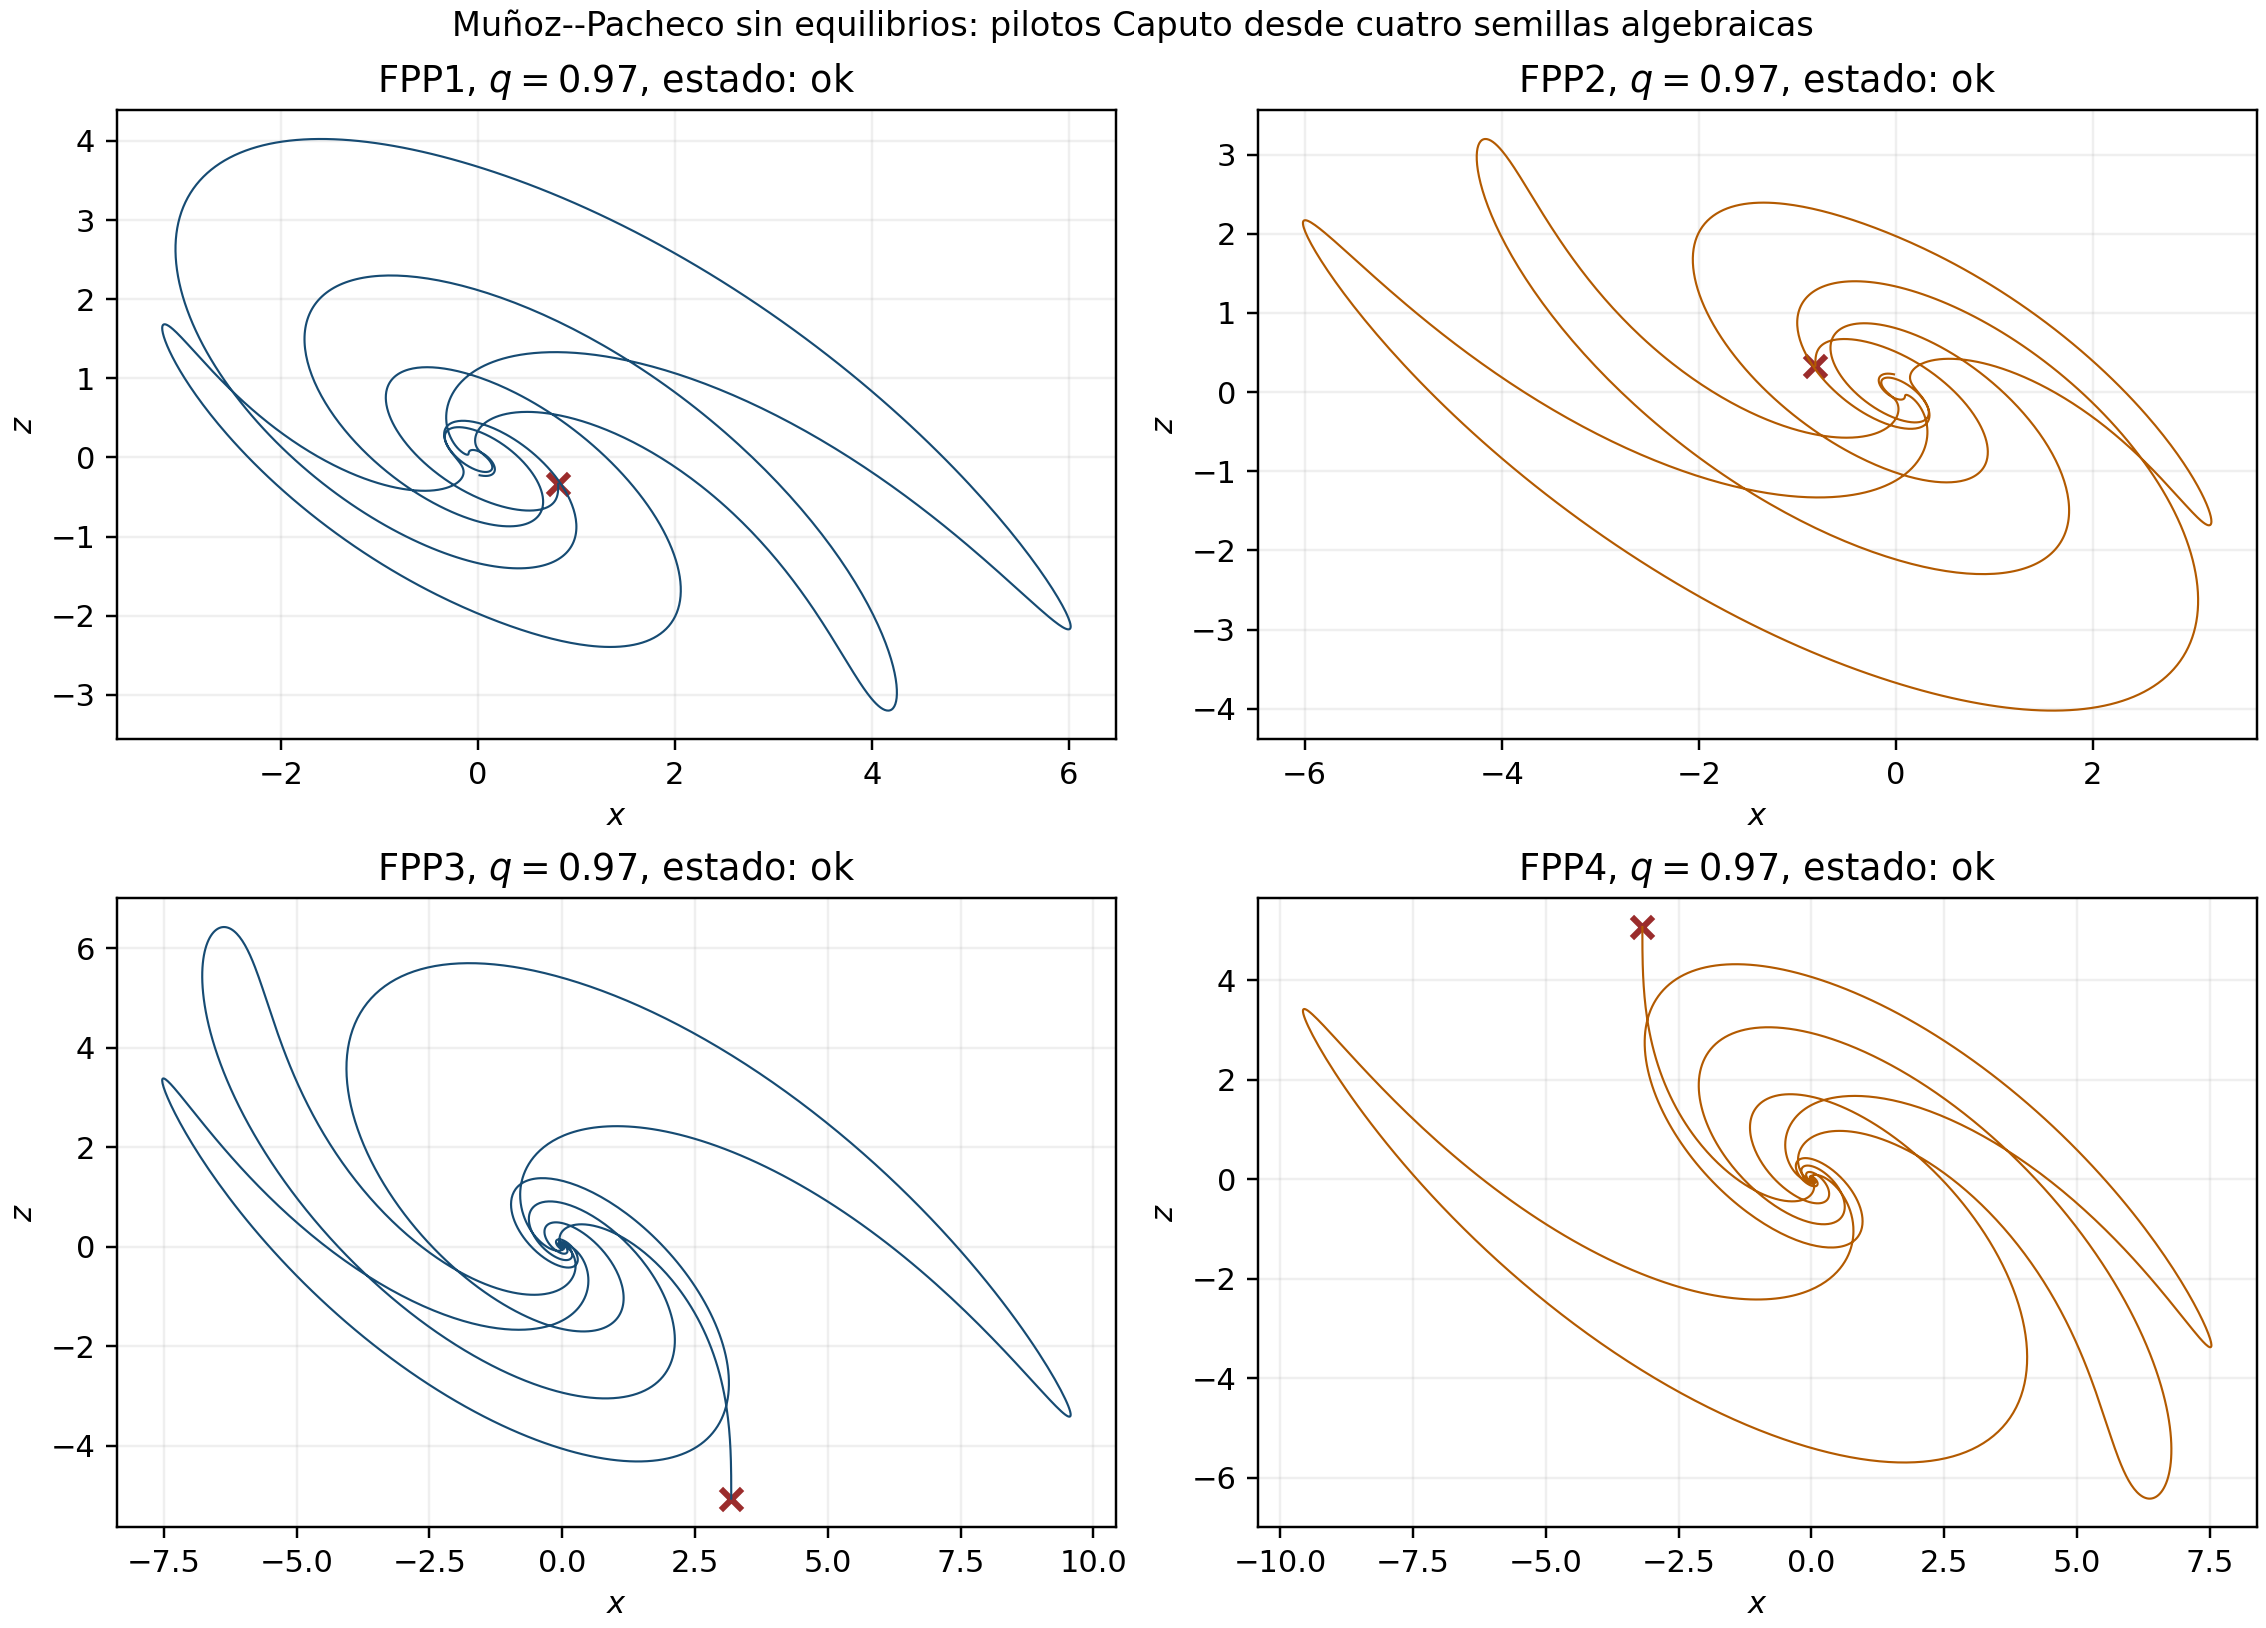
\includegraphics[width=0.96\linewidth]{figures/perpetual/perpetual_munoz_caputo.png}
 \caption{Experimento Caputo desde las cuatro semillas FPP--A exactas de
 Muñoz--Pacheco. Las cruces indican el estado inicial. Las curvas muestran
 trayectorias finitas, no una afirmación de atracción ni ocultedad.}
 \label{fig:pp-munoz-pilot}
\end{hafodigitalfigure}

Para FPP1 se calculó además \cref{eq:fpph-l1}. En el horizonte común
\([2,17.5]\), las curvas \(h=0.01\) y \(h=0.005\) concuerdan cualitativamente,
pero ningún mínimo converge a cero: el refinamiento dio un mínimo normalizado
aproximado \(0.0871\) cerca de \(t=11.965\). La corrida gruesa alcanzó
\(0.0254\) en \(t=32.33\), fuera del horizonte fino, y por eso no se clasifica
como evento FPP--H. El panel de arranque sí muestra que el cociente de
\cref{eq:pp-startup-limit} decrece hacia el residuo algebraico cero al refinar
\(h\).

\begin{hafodigitalfigure}[H]
 \centering
 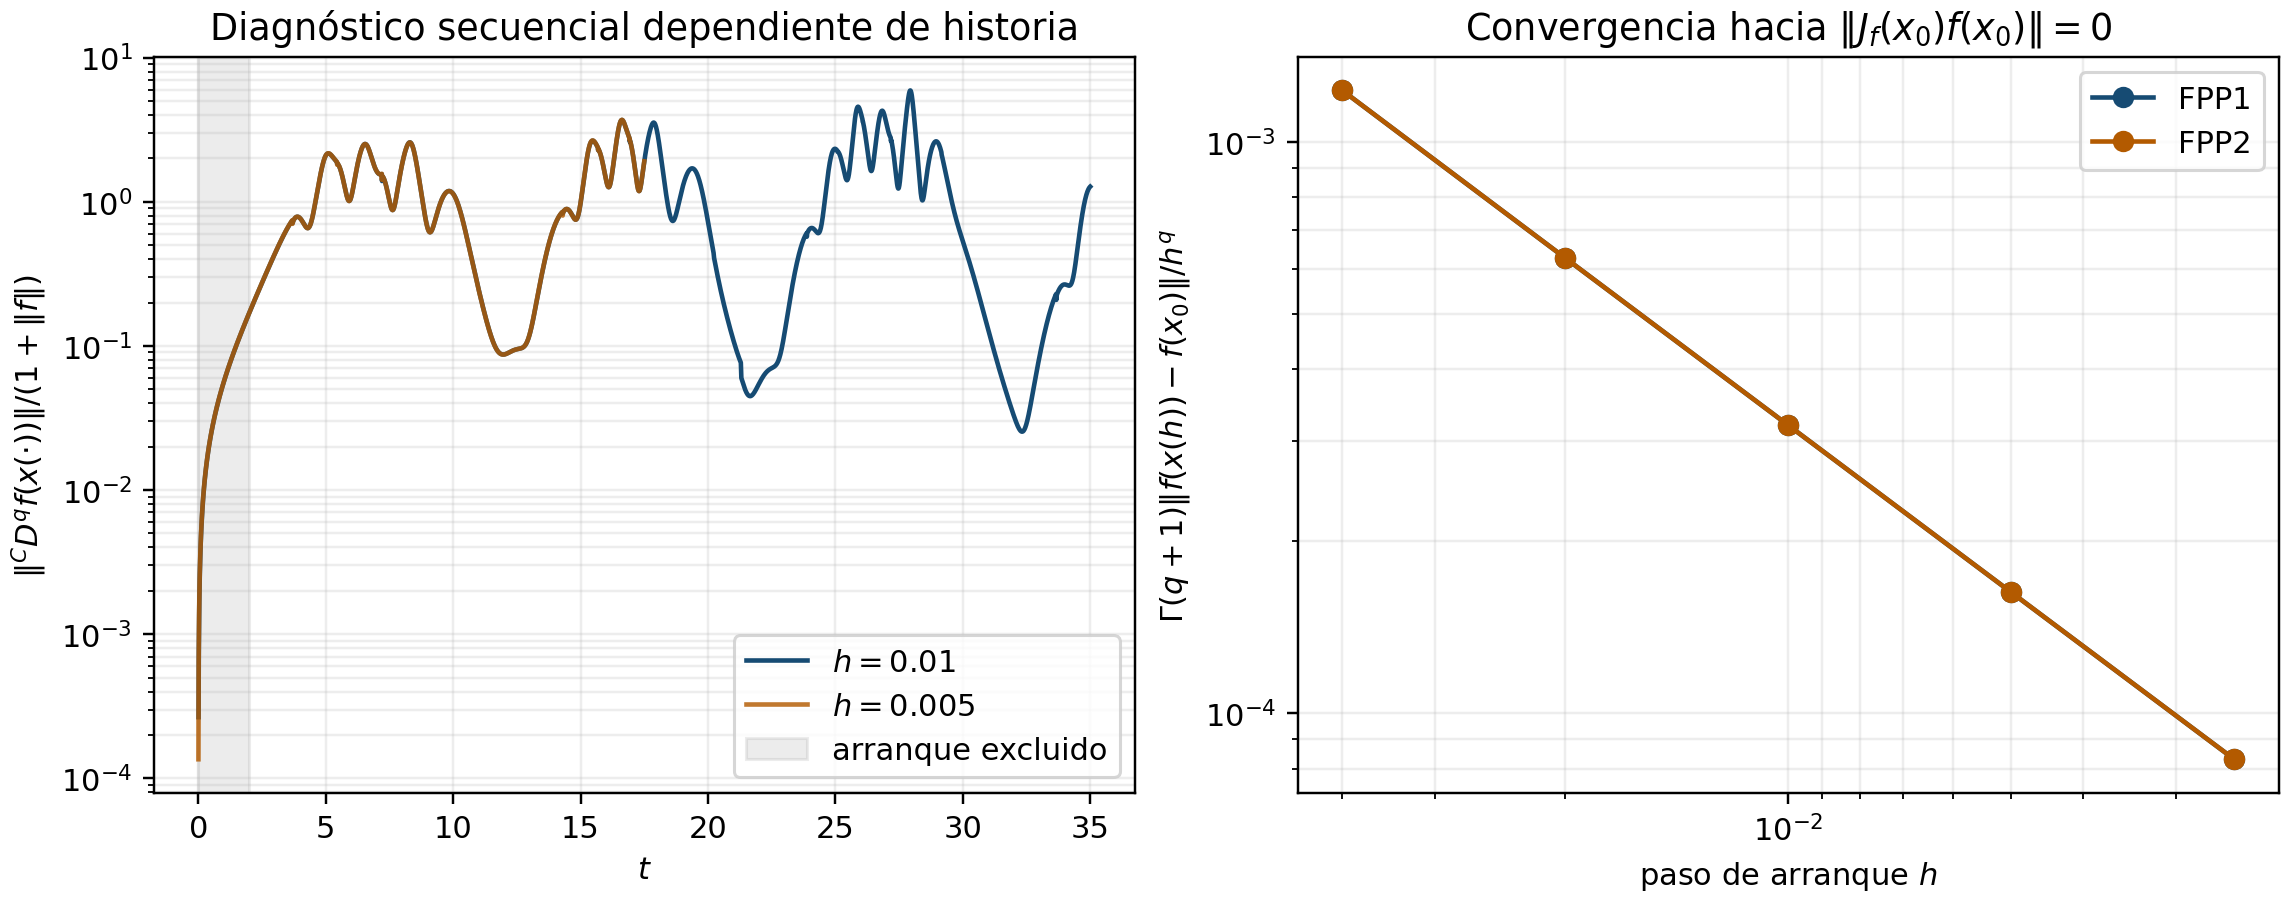
\includegraphics[width=0.98\linewidth]{figures/perpetual/perpetual_caputo_history_diagnostics.png}
 \caption{Izquierda: aceleración secuencial L1 dependiente de historia; el
 intervalo gris se excluye por arranque. Derecha: verificación numérica del
 límite de arranque en dos raíces simétricas. La ausencia de un cero
 convergente impide reclamar un evento FPP--H.}
 \label{fig:pp-caputo-history}
\end{hafodigitalfigure}

\subsubsection{Chua arctangente}

Escribiendo \(h(x)=a_1x+a_2\arctan(\rho x)\), la condición singular produce
la primera restricción sobre la coordenada \(x\). En efecto, el campo y su
Jacobiano son
\[
 f=\begin{pmatrix}\alpha(y-x-h(x))\\x-y+z\\-\beta y-\gamma z\end{pmatrix},
 \qquad
 J_f=\begin{pmatrix}
 -\alpha(1+h'(x))&\alpha&0\\1&-1&1\\0&-\beta&-\gamma
 \end{pmatrix}.
\]
Si \(U=f_1\), las dos primeras filas de \(J_ff=0\) imponen
\(f_2=(1+h')U\) y \(f_3=h'U\). Un PP requiere \(U\ne0\), porque
\(U=0\) anularía también \(f_2,f_3\). La tercera fila se reduce a
\([\beta+(\beta+\gamma)h']U=0\). Para
\(\alpha\rho(\beta+\gamma)\ne0\), se obtiene
\begin{equation}
 h'(x_\star)=-\frac{\beta}{\beta+\gamma},
 \quad
 x_\star^2=\frac1{\rho^2}
 \left[
 \frac{a_2\rho}{-\beta/(\beta+\gamma)-a_1}-1
 \right],
 \label{eq:pp-chua-arctan-x}
\end{equation}
si el miembro derecho es positivo. El denominador
\(-\beta/(\beta+\gamma)-a_1\) debe ser no nulo. Si se anula, se vuelve a
\(h'(x)=a_1+a_2\rho/(1+\rho^2x^2)\): para \(a_2\rho\ne0\) no hay
solución finita; para \(a_2\rho=0\) la restricción singular se satisface
en toda la recta y se debe resolver el sistema lineal restante sin
dividir. Este caso degenerado no aparece en Wu ni en c590. Un valor negativo del
miembro derecho excluye raíces reales. Para un valor cero se comprueba
\(x_\star=0\) en el sistema original. Dado uno de los signos admisibles,
escriba \(p=h'(x_\star)\). Las identidades
\(f_1=U\), \(f_2=(1+p)U\) dan sucesivamente
\[
 y_\star=x_\star+h(x_\star)+U/\alpha,
 \qquad
 z_\star=h(x_\star)+(1+p)U+U/\alpha.
\]
Al sustituirlas en \(-\beta y_\star-\gamma z_\star=pU\), resulta la
ecuación lineal
\[
 \left[\gamma+(1+\gamma)p+\frac{\beta+\gamma}{\alpha}\right]U
 =-\beta x_\star-(\beta+\gamma)h(x_\star).
\]
Por tanto,
\begin{equation}
 U=-\frac{\beta x_\star+(\beta+\gamma)h(x_\star)}
 {\gamma+(1+\gamma)p+(\beta+\gamma)/\alpha},
\end{equation}
si el coeficiente de \(U\) es no nulo. Si se anula, se resuelve la
ecuación lineal anterior sin dividir: un término derecho no nulo descarta
la raíz; si ambos se anulan, queda una familia que debe comprobarse en
\(J_ff=0\). Finalmente se exige \(U\ne0\). En los casos Wu y c590 los
denominadores son no nulos y ambos signos producen PP; la imparidad de
\(h\) relaciona las dos raíces por simetría central.
Para Wu con \(q=0.99\), las raíces son
\begin{equation}
 \pm(0.3369817810952544, 0.0815749282686440,
 -0.2549832342782550),\qquad \|f\|=1.39124162716.
\end{equation}
Para c590, \(q=0.9999\), el par es
\begin{equation}
 \pm(1.213090022614086, -20.18726992409549,
 -21.54936334065727),\qquad \|f\|=545.09983035.
\end{equation}
La gran norma y la distancia al conjunto observado en c590 obligan a
controlar el transitorio y el escape antes de usar el segundo par como
semilla. En Wu, las integraciones de ambos signos permanecen acotadas, pero
no resuelven un destino asintótico común; véase
\cref{sec:resultados-piloto-gt}.

\subsubsection{Chua PWL y Kalman--Fitts como controles negativos}

En una región de pendiente \(m\), el Jacobiano de Chua PWL satisface
\begin{equation}
 \det J_m=-\alpha[\beta+(\beta+\gamma)m].
 \label{eq:pp-chua-pwl-det}
\end{equation}
Con \(m_0=-0.1768\) y \(m_1=-1.1468\), los valores son
\(-84.035507517056\) y \(15.037737580544\). Al ser invertibles, cada región
sólo admite equilibrios en \(J_mf=0\). En \(x=\pm1\), la derivada
direccional usa uno de esos Jacobianos si \(f\) apunta a una región;
si es tangente, ambos productos coinciden por continuidad del campo PWA.
En cualquiera de los casos, la invertibilidad excluye un producto cero
con \(f\ne0\). La función descriptiva y la
continuación localizan órbitas donde PP no genera semilla.

En Kalman--Fitts, \(f(X)=AX+e_4\tanh(-X_3/\varepsilon)\), la
derivada de \(\tanh\) sólo modifica la tercera entrada de la última
fila de la matriz compañera \(A\). Su determinante, igual al coeficiente
constante del polinomio característico, permanece inalterado:
\begin{equation}
 \det J_f=0.98191881\neq0.
\end{equation}
Por \cref{eq:pp-singular-screen}, no existe PP. El mapa de conmutación
proporciona una vía alternativa de localización.

\subsubsection{Ausencia de puntos perpetuos en los dos sistemas jerk}
\label{subsec:pp-jerk-exclusion}

\begin{proposition}[jerk cuadrático y jerk exponencial]
\label{prop:pp-jerk-exclusion}
Los campos de \cref{eq:cand-jerk,ncbench:eq:jerk} no tienen puntos perpetuos
no estacionarios. El jerk exponencial tampoco tiene semillas FPP--A para
ningún orden conmensurable \(0<q<1\).
\end{proposition}

\begin{proof}
En un campo jerk \(f=(y,z,G(x,y,z))^{\mathsf T}\),
\begin{equation}
 J_ff=\bigl(z,G,G_xy+G_yz+G_zG\bigr)^{\mathsf T}.
 \label{eq:pp-jerk-general-acceleration}
\end{equation}
Por tanto, toda raíz satisface \(z=G=0\) y \(G_xy=0\).
Para el jerk cuadrático,
\[
 G=-x-y-1.1z-2.59z^2+xy,\qquad G_x=y-1.
\]
La última condición se reduce a \(y(y-1)=0\). Si \(y=0\), las otras
dos ecuaciones dan \(z=x=0\), el equilibrio. Si \(y=1\), entonces
\(G(x,1,0)=-1\), incompatible con \(G=0\). Estas dos ramas agotan las
posibilidades reales.

Para el jerk exponencial,
\[
 G=-az-I_c\left(e^{y/(nV_T)}-1\right)-x,\qquad G_x=-1.
\]
Así, \(G_xy=0\) obliga a \(y=0\), y \(z=G=0\) obliga a \(x=0\).
Equivalentemente, \(\det J_f=G_x=-1\) en todo \(\mathbb R^3\).
Ambos campos son suaves y no hay regiones ni fronteras adicionales que
examinar. La condición FPP--A conmensurable es la misma ecuación
\(J_ff=0\), con los equilibrios excluidos.
\end{proof}

Esta ausencia limita la generación de semillas por PP. No excluye
atractores ni eventos FPP--H a lo largo de una historia.

\subsubsection{PLL lead--lag}

En las coordenadas publicadas \((x,\theta)\), con
\(T=\tau_1+\tau_2>0\), el campo es
\[
 f_x=-\frac{x}{T}+\frac{\tau_1}{2T}\sin\theta,\qquad
 f_\theta=\omega_\Delta-\frac{Lx}{T}
                         -\frac{\tau_2L}{2T}\sin\theta.
\]
Derivar sus dos componentes y tomar el determinante da
\begin{equation}
 \det J_f=\frac{L\cos\theta}{2(\tau_1+\tau_2)}.
\end{equation}
Como un PP tiene \(f\ne0\), la singularidad del Jacobiano exige
\(\cos\theta=0\). En esos ángulos,
\[
 J_f=\begin{pmatrix}-1/T&0\\-L/T&0\end{pmatrix},\qquad
 T=\tau_1+\tau_2>0.
\]
Así, \(J_ff=0\) equivale a \(f_x=0\), es decir,
\(x=\tau_1\sin\theta/2\). La otra componente se reduce a
\(f_\theta=\omega_\Delta-L\sin\theta/2\).
Los PP por vuelta del cilindro son
\begin{equation}
 \left(\frac{\tau_1}{2},\frac\pi2\right),
 \qquad
 \left(-\frac{\tau_1}{2},\frac{3\pi}{2}\right),
 \label{eq:pp-pll}
\end{equation}
si las velocidades angulares correspondientes
\(\omega_\Delta\mp L/2\) no se anulan. Numéricamente son
\((0.0224,1.5707963268)\), con \(f=(0,-71.1)\), y
\((-0.0224,4.7123889804)\), con \(f=(0,428.9)\). La comparación debe usar
distancia cilíndrica y las mismas coordenadas, por
\cref{eq:pp-nonlinear-coordinate}. En las integraciones de
\cref{sec:resultados-piloto-gt}, la semilla positiva llega al foco y la
negativa permanece como un transitorio acotado sin destino resuelto.

\subsubsection{Lorenz generalizado y Rabinovich--Fabrikant}

Para el Lorenz generalizado,
\begin{equation}
 f=\begin{pmatrix}
 -\sigma(x-y)-ayz\\rx-y-xz\\-z+xy
 \end{pmatrix},\qquad
 J_f=\begin{pmatrix}
 -\sigma&\sigma-az&-ay\\r-z&-1&-x\\y&x&-1
 \end{pmatrix}.
\end{equation}
Con \((r,a,\sigma)=(6.8,-0.5,3.4)\), el sistema \(J_ff=0\) tiene cinco raíces
reales. Para obtenerlas sin confundir equilibrios y PP, se parte de las
componentes explícitas de \cref{casegt:eq:lorenz-A}. Si \(x=0\) y
\(y\ne0\), las dos primeras exigirían simultáneamente
\(z=-748/135\) y \(z^2=1206/25\), lo cual es imposible. Si
\(y=0\) y \(x\ne0\), exigirían \(z=748/135\) y
\(z^2=1734/25\), también incompatibles. Cuando \(x=y=0\), la tercera
componente da \(z=0\). Toda raíz restante tiene \(xy\ne0\).

Introduzca \(u=x^2>0\) y \(v=y/x\ne0\). Al dividir las dos primeras
ecuaciones entre \(x\), el sistema equivale a
\begin{equation}
 \frac{v^2}{2}u+c_1(v,z)=0,\qquad
 -vu+c_2(v,z)=0,\qquad u c_3(v,z)+z=0,
 \label{eq:pp-lorenz-reduced-three}
\end{equation}
donde
\begin{align}
 c_1&=\frac{867}{25}-\frac{374}{25}v-\frac{27}{10}vz-\frac12z^2,\nonumber\\
 c_2&=-\frac{748}{25}+\frac{603}{25}v+\frac{27}{5}z-\frac12vz^2,\\
 c_3&=\frac{34}{5}-\frac{27}{5}v+\frac{17}{5}v^2
       +\left(\frac{v^2}{2}-1\right)z.
 \label{eq:pp-lorenz-c-polynomials}
\end{align}
La segunda ecuación da \(u=c_2/v\). Sustituirla en las otras dos produce
\begin{align}
 L(v,z)&=\frac{3468-2992v+1206v^2}{25}-(2+v^2)z^2=0,\nonumber\\
 Q(v,z)&=vz+c_2(v,z)c_3(v,z)=0.
 \label{eq:pp-lorenz-two-polynomials}
\end{align}
El resultante respecto de \(v\), definido como el determinante de la
matriz de Sylvester de estos dos polinomios, factoriza como
\begin{equation}
 \operatorname{Res}_v(L,Q)
 =-5^{-12}(25z^2-1206)(25z^2-986)P_L(z),
 \label{eq:pp-lorenz-resultant}
\end{equation}
con
\begin{align}
 P_L(z)={}&781250z^8-94421875z^6-112200000z^5\nonumber\\
 &+3621441250z^4+6045336000z^3-60977294900z^2\nonumber\\
 &-150632718720z-231894425384.
 \label{eq:pp-lorenz-eliminant}
\end{align}
Para reconstruir \(v\), la división de \(Q\) entre \(L\) respecto de
\(v\) deja el resto
\[
 \frac{R_1(z)v+R_0(z)}{125(25z^2-1206)},
\]
donde
\begin{align}
 R_0(z)&=18307572+4398240z+2697400z^2-50625z^4,\nonumber\\
 R_1(z)&=-2864840+647540z-1739100z^2-422500z^3+3125z^5.
 \label{eq:pp-lorenz-reconstruction-polynomials}
\end{align}
Las raíces de \((25z^2-986)P_L\) no anulan \(R_1\), pues el máximo
común divisor de ambos polinomios es uno. En ellas,
\begin{equation}
 v=-R_0/R_1,\qquad u=c_2/v,\qquad
 x=\pm\sqrt u,\quad y=vx.
 \label{eq:pp-lorenz-reconstruction}
\end{equation}
El factor \(25z^2-1206\) corresponde a una caída de grado en \(L,Q\);
al sustituir \(z^2=1206/25\), la ecuación \(L=0\) exige
\(v=66/187\), pero
\[
 \gcd\bigl(25z^2-1206,Q(66/187,z)\bigr)=1
\]
tras eliminar denominadores. Sus dos raíces se descartan antes de usar
la fórmula racional. Fuera de esa rama, el coeficiente principal de
\(L\), respecto de \(v\), no se anula. La anulación del resultante
equivale entonces a una raíz común de \(L\) y su resto lineal; esto
justifica el levantamiento \(v=-R_0/R_1\), además de su unicidad.

Para contar raíces reales, la sucesión de Sturm se construye con
\(S_0=P\), \(S_1=P'\) y
\(S_{j+1}=-\operatorname{rem}(S_{j-1},S_j)\), hasta el último resto no
nulo. Sea \(V_P(t)\) el número de cambios de signo de la sucesión evaluada
en \(t\), omitiendo ceros. La diferencia \(V_P(a)-V_P(b)\) cuenta las
raíces distintas en \((a,b)\), si sus extremos no son raíces. Para \(P_L\),
\[
 \begin{array}{c|rrrrrr}
 t&-\infty&-7.443&-7.442&9.321&9.322&+\infty\\\hline
 V_{P_L}(t)&5&5&4&4&3&3
 \end{array}
\]
Los extremos decimales son racionales exactos. Hay una raíz en cada
intervalo indicado y ninguna otra raíz real. Las condiciones de
reconstrucción separan las ramas:
\begin{center}
\begin{tabular}{@{}rrrr@{}}
\toprule
\(z\) & \(v\) & \(u=x^2\) & Admisibilidad\\\midrule
\(-6.2801273872\) & \(13.0801273872\) & \(-0.4801273872\) & no real\\
\(6.2801273872\) & \(0.5198726128\) & \(12.0801273872\) & equilibrio\\
\(-7.4423053062\) & \(-16.9736823118\) & \(0.5564665577\) & PP\\
\(9.3218987982\) & \(-0.3277828328\) & \(-81.6209147361\) & no real\\
\bottomrule
\end{tabular}
\end{center}
La admisibilidad no depende del redondeo de la tabla. La forma equivalente
\begin{equation}
 u=\frac{603}{25}-\frac{z^2}{2}
   +\frac{-748/25+27z/5}{v}
 \label{eq:pp-lorenz-sign-certificate}
\end{equation}
permite evaluar con aritmética racional de intervalos: para la raíz de
\(P_L\) en \((-7.443,-7.442)\), se obtiene \(0.29<u<0.83\); para la
raíz en \((9.321,9.322)\), se obtiene \(-82<u<-81\).
Los denominadores quedan separados de cero en ambos intervalos.
Para \(25z^2-986=0\), la reconstrucción da exactamente \(u=29/5+z\);
la raíz positiva admite \(u>0\), mientras la negativa cumple
\(z<-29/5\) y obliga a \(u<0\).
La fila de equilibrio reconstruye el par de \cref{nc:eq:lorenz-eq1}; la
fila PP reconstruye
\begin{equation}
 (-0.745966861002653, 12.66180451381419, -7.442305306160726)
\end{equation}
y su imagen por \((x,y,z)\mapsto(-x,-y,z)\), con
\(\|f\|=23.42210895339\). Son candidatos FPP--A para \(q=0.995\), pero aún no
cuentan con validación dinámica.

Para Rabinovich--Fabrikant,
\begin{align}
 f_1&=y(z-1+x^2)+ax,\\
 f_2&=x(3z+1-x^2)+ay,\\
 f_3&=-2z(b+xy),
\end{align}
y
\begin{equation}
 J_f=\begin{pmatrix}
 2xy+a&z-1+x^2&y\\
 3z+1-3x^2&a&3x\\
 -2yz&-2xz&-2(b+xy)
 \end{pmatrix}.
 \label{eq:pp-rf-jacobian}
\end{equation}
Para \((a,b)=(1/10,719/2500)\), se separan primero los casos \(x=0\)
y \(z=0\). Si \(x=0\), las aceleraciones primera y tercera son
\[
 A_1=2y[(a-b)z-a],\qquad
 A_3=2z[2b^2-y^2(z-1)].
\]
Si \(y=0\), \(A_3=0\) obliga a \(z=0\). Si \(y\ne0\), la primera
ecuación obliga a \(z=a/(a-b)<0\); entonces la segunda exigiría
\(y^2(z-1)=2b^2>0\), imposible. Por tanto, la única raíz con \(x=0\)
es el origen.

Para \(x\ne0\), introduzca \(u=x^2>0\), \(v=xy\) y
\(H=u+z-1\), \(K=3z+1-u\). La multiplicación explícita de
\cref{casegt:eq:rf-A} da
\begin{align}
 E_1:=xA_1&=u(a^2+HK)+2v[a(u+H)-bz]+2(u-1)v^2,\nonumber\\
 E_2:=xA_2&=D(u,z)v+C(u,z),\label{eq:pp-rf-reduced-three}\\
 -\frac{uA_3}{2z}&=E_3:=(z-1-u)v^2+2u(a-2b)v+u(uK-2b^2),\nonumber
\end{align}
donde la última igualdad se usa sólo para \(z\ne0\), y
\begin{align}
 D&=3z^2-6uz-2z-3u^2+4u+a^2-1,\nonumber\\
 C&=2u[a(3z+1-2u)-3bz].
 \label{eq:pp-rf-D-C}
\end{align}

En el plano \(z=0\), \(A_3\) se anula idénticamente y basta resolver
\(E_1=E_2=0\). La eliminación de \(v\) da
\begin{align}
 \operatorname{Res}_v(E_1|_{z=0},E_2|_{z=0})
 ={}&-10^{-6}u(10u-11)(10u-9)\nonumber\\
 &\times[100(u-1)^2+1][100(3u-1)^2+1].
 \label{eq:pp-rf-z0-resultant}
\end{align}
Los factores cuadráticos son estrictamente positivos. Como \(u>0\), las
únicas posibilidades son
\[
 (u,v)=(9/10,4/5),\qquad (u,v)=(11/10,-6/5).
\]
Sustituir estos pares en \(E_1,E_2\) da cero y reconstruye cuatro PP
mediante \(x=\pm\sqrt u\), \(y=v/x\). Ninguno es un equilibrio:
en \(z=0\), el sistema \(f_1=f_2=0\) tiene determinante
\(a^2+(u-1)^2>0\) y sólo admite \(x=y=0\).

Para \(z\ne0\), se resuelven las tres ecuaciones \(E_j=0\).
Antes de dividir entre \(D\), se comprueba su rama excepcional. Si
\(D=0\), \(E_2=0\) exige \(C=0\); por \(u>0\),
\[
 u=u_D(z):=\frac{1250-7035z}{2500},\qquad
 d_D(z):=65000-1953500z-967947z^2=0.
\]
Al sustituir \(u_D\) en \(E_1,E_3\), se obtiene
\[
 \gcd\!\left(d_D,
 \operatorname{Res}_v(E_1(u_D,v,z),E_3(u_D,v,z))\right)=1,
\]
tras eliminar denominadores constantes. No hay una raíz común y la rama
\(D=0\) queda excluida. Para \(D\ne0\), \(v=-C/D\). Al multiplicar
por \(D^2\), las otras dos ecuaciones equivalen a
\begin{align}
 P(u,z)={}&u(a^2+HK)D^2-2CD[a(u+H)-bz]+2(u-1)C^2=0,\nonumber\\
 Q(u,z)={}&(z-1-u)C^2-2u(a-2b)CD+u(uK-2b^2)D^2=0.
 \label{eq:pp-rf-P-Q}
\end{align}
Defina los polinomios
\[
 S(u)=32264900u^2-215503200u+82528417,\qquad
 E(u)=53150000u^2-71900000u+516961.
\]
El resultante de \(P,Q\) respecto de \(z\) es un múltiplo constante
no nulo de \(u^{13}S(u)^4E(u)P_R(u)\). Una definición exacta y compacta
del factor de grado catorce es
\begin{equation}
 P_R(u)=\operatorname{pp}\!\left(
 \frac{\operatorname{Res}_z(P,Q)}{u^{13}S(u)^4E(u)}\right),
 \label{eq:pp-rf-eliminant}
\end{equation}
donde \(\operatorname{pp}\) elimina denominadores y el máximo común divisor
de los coeficientes, y fija positivo el coeficiente principal. Todas las
entradas del determinante de Sylvester están dadas en
\cref{eq:pp-rf-D-C,eq:pp-rf-P-Q}; no se requiere una aproximación numérica
para definir \(P_R\).

Para la evaluación directa, escriba
\(P_R(u)=\sum_{k=0}^{14}m_k10^{e_k}u^k\), con coeficientes enteros:
\begin{center}
\small
\begin{tabular}{@{}rrr@{}}
\toprule
\(k\)&\(m_k\)&\(e_k\)\\\midrule
0&172890165175624363345259174569803&0\\
1&14469699682074574386521765557812&2\\
2&\(-18396580138862579542741337855542518\)&2\\
3&15478807059059016799618863592551164&4\\
4&\(-483305962260027081263570393541627373\)&4\\
5&56915116746512318338898887806915&9\\
6&\(-1629237154908128789498842947039615\)&8\\
7&95325977171002410189945625&14\\
8&125564435311034818006205569375&13\\
9&\(-433337883019314447578125\)&19\\
10&81563269511051918346484375&17\\
11&\(-99102930618837890625\)&23\\
12&77980731527669677734375&20\\
13&\(-358729705810546875\)&25\\
14&722605133056640625&24\\\bottomrule
\end{tabular}
\end{center}

La raíz \(u=0\) pertenece al caso ya separado. Las raíces de \(S\)
provienen de la eliminación de denominadores: al reducir \(P,Q\) con
\(S=0\), sus raíces comunes con \(u>0\) cumplen \(D=C=0\), rama
excluida antes de la división. Las dos raíces positivas de
\(E\) reconstruyen los cuatro equilibrios no nulos de
\cref{nc:eq:rf-e12,nc:eq:rf-e34}, con \(v=-b\). Para comprobar esta
identificación, \(f_3=0\), \(z\ne0\), exige \(v=-b\);
de \(xf_1=au+vH=0\) se obtiene \(z=1-u+au/b\).
La ecuación \(xf_2=uK+av=0\) queda
\[
 (4b-3a)u^2-4bu+ab^2=0.
\]
Multiplicarla por \(62500000\) produce exactamente \(E(u)=0\).
Su discriminante es positivo y tanto la suma como el producto de las
raíces son positivos; ambas son reales positivas. Cada una reconstruye
dos signos de \(x\), y la sustitución verifica las tres componentes del
campo. Queda \(P_R\), cuya
sucesión de Sturm da
\[
 \begin{array}{c|rrrrrr}
 t&0&0.0391&0.0392&0.0474&0.0475&+\infty\\\hline
 V_{P_R}(t)&7&7&6&6&5&5
 \end{array}
\]
Hay exactamente dos raíces positivas. El levantamiento desde \(u\) se
justifica mediante una forma triangular exacta. Sea \(Z(u)\) el
polinomio racional de grado trece definido por la base de Gröbner reducida
y mónica del ideal \(\langle P,Q,P_R\rangle\), con orden lexicográfico
\(z>u\). Esa base es
\begin{equation}
 \left\{\frac{P_R(u)}{\operatorname{lc}(P_R)},\ z-Z(u)\right\},
 \qquad \deg Z=13,
 \label{eq:pp-rf-triangular}
\end{equation}
donde \(\operatorname{lc}\) denota el coeficiente principal. Esta
definición usa exclusivamente los coeficientes racionales de
\cref{eq:pp-rf-P-Q,eq:pp-rf-eliminant} y fija \(Z\) de manera única.
La división polinómica proporciona los certificados
\begin{align}
 P(u,Z(u))&\equiv Q(u,Z(u))\equiv0\pmod{P_R(u)},\nonumber\\
 \gcd(P_R,Z)&=\gcd\bigl(P_R,D(u,Z)\bigr)=1,\nonumber\\
 \gcd\bigl(P_R,bD(u,Z)-C(u,Z)\bigr)&=1,
 \label{eq:pp-rf-lifting-certificates}
\end{align}
normalizando cada máximo común divisor a mónico. Por la igualdad de
ideales de \cref{eq:pp-rf-triangular}, cada raíz de \(P_R\) tiene
exactamente un levantamiento \(z=Z(u)\). Para las dos raíces reales
positivas, \(Z(u)\) es real; los dos primeros máximos comunes divisores
excluyen \(z=0\) y \(D=0\). Se reconstruye entonces
\begin{equation}
 v=-C/D,\qquad x=\pm\sqrt u,\qquad y=v/x.
 \label{eq:pp-rf-reconstruction}
\end{equation}
Los dos triples reducidos son
\[
 \begin{array}{c|rr}
 u&v&z\\\hline
 0.0391007463043&-0.0447439313091&0.822145202941\\
 0.0474835273591& 0.0710968429474&1.202380810759
 \end{array}
\]
y ambos tienen \(v\ne-b\): si \(v=-C/D=-b\), se anularía
\(bD-C\), contradiciendo el último certificado de
\cref{eq:pp-rf-lifting-certificates}. Así,
\(f_3=-2z(b+v)\ne0\) y ninguno es un equilibrio.
Las cuatro raíces del plano \(z=0\), estas cuatro raíces y los cinco
equilibrios agotan las trece soluciones reales de \(J_ff=0\). Cuatro
representantes de los ocho PP son
\begin{align}
 &( -1.04880884817015, 1.14415510709471, 0),\\
 &( 0.948683298050514, 0.843274042711568, 0),\\
 &( 0.217907153070161, 0.326271267123146, 1.202380810758825),\\
 &( -0.197739086435437, 0.226277627330655, 0.822145202940591),
\end{align}
más sus imágenes por \((x,y,z)\mapsto(-x,-y,z)\). Las normas del campo son,
respectivamente, \(0.21950,0.17951,1.34455,0.76891\). Antes de una corrida
Caputo \(q=0.998\) se deduplican los cuatro pares y se asigna el mismo
presupuesto a cada uno.

\subsection{Protocolo de validación PP0--PP5}

\begin{description}[style=nextline,leftmargin=3.2em,labelwidth=2.7em]
 \item[PP0] Fijar fuente, campo, coordenadas, parámetros, dominio y
 convención no suave.
 \item[PP1] Calcular \(J_f\), \(J_f f\), \(\det J_f\); resolver raíces reales,
 excluir \(\|f\|\leq\nu\), verificar región y evaluar el residuo con
 50 dígitos de precisión.
 \item[PP2] En entero, integrar desde cada PP, perturbaciones radiales
 \(10^{-6},10^{-4},10^{-2}\) y controles aleatorios de igual norma, con la
 configuración analizada.
 \item[PP3] En Caputo, distinguir FPP--A de FPP--H; usar historia completa como
 oráculo, terminal inferior común, \(h,h/2\) y una réplica corta \(h/4\).
 \item[PP4] Clasificar destino, recurrencia, robustez y, para FPP--H, mínimos de
 \(\eta_{q,n}\); separar continuación con historia y reset desde el estado.
 \item[PP5] Reutilizar los sondeos de todos los equilibrios y el primer
 contacto. Llegar al conjunto desde un PP no demuestra ocultedad.
\end{description}

Para Muñoz--Pacheco no hay equilibrios; la condición usual de cuenca separada
de vecindades de equilibrios es vacua. El experimento evalúa capacidad de
localización y coexistencia, no distingue por sí solo entre autoexcitación y
ocultedad. El control de Nag Chowdhury--Ghosh debe acompañar cualquier
afirmación de generalidad.

\subsection{Complementariedad de los métodos}

\begin{longtable}{@{}L{0.20\linewidth}L{0.31\linewidth}L{0.39\linewidth}@{}}
\caption{Funciones complementarias en la localización.}
\label{tab:method-complementarity}\\
\toprule
Método & Qué aporta & Qué no demuestra\\
\midrule
\endfirsthead
\toprule
Método & Qué aporta & Qué no demuestra\\
\midrule
\endhead
DF clásica/sesgada & Semillas armónicas estructuradas en Lur'e; cierre DC y
fundamental & Existencia exacta del ciclo Caputo, caos u ocultedad.\\
Machado & Barrido de amplitudes/órdenes auxiliares y DF complejos con rama
declarada & Que \(N^\mu\) sea el Fourier físico de la no linealidad original.\\
Balance MIMO & Semillas para campos no reducibles a un canal & Convergencia de
armónicos omitidos sin una prueba de truncación.\\
FPP--A & Raíces algebraicas para campos generales y cancelación del segundo
término Picard & Aceleración fraccionaria global o pertenencia a una cuenca.\\
FPP--H & Eventos dependientes de historia sobre trayectorias ya calculadas &
Un punto de estado independiente de la prehistoria.\\
Continuación & Transporte de una rama o trayectoria entre parámetros y
órdenes & Ocultedad si no se congela el campo final y se sondean cuencas.\\
Sondeo de cuenca & Evidencia finita de separación respecto de equilibrios &
Prueba topológica global con un número finito de condiciones.\\
\bottomrule
\end{longtable}

La búsqueda usa la \emph{unión} de semillas. Para cada caso se
compara, con igual presupuesto, DF clásica, DF sesgada, Machado, balance MIMO,
FPP--A y controles aleatorios; la continuación transporta las supervivientes;
FPP--H diagnostica la historia; y los sondeos de cuenca conservan el nivel
probatorio final. La comparación no establece superioridad universal de un
método.

\subsection{Condiciones de aplicación de las extensiones fraccionarias}

\begin{proposalbox}
FPP--A cancela el coeficiente \(h^{2q}\) de la expansión Picard--Caputo y
se comprueba mediante \cref{eq:pp-startup-limit}. FPP--H requiere existencia
y regularidad de \cref{eq:fpph-history-integral}, un terminal inferior común
y convergencia al refinar la discretización de la historia. La comparación
con el PVI reiniciado determina el efecto de la memoria. Ninguna de estas
condiciones sustituye el estudio de la cuenca del destino localizado.
\end{proposalbox}

MAVPD \(q=1\) proporciona un control de localización;
Chua PWL, Kalman--Fitts y los dos jerk son controles algebraicos sin PP. Muñoz--Pacheco
\(q=0.97\) permite contrastar FPP--A y FPP--H; Lorenz
\(q=0.995\) y RF \(q=0.998\) proporcionan semillas multicanal cuyo destino
debe determinarse. Wu \(q=0.99\) permite comparar integradores con memoria
completa, y c590 exige controlar el efecto de semillas lejanas.
